\documentclass[journal,onecolumn]{IEEEtran}
\usepackage{amsmath}
\usepackage{amssymb}
\usepackage{algorithm, algorithmic}
\interdisplaylinepenalty=2500
\usepackage{algorithmic, algorithm}
\usepackage{array}
\linespread{2.0}
\usepackage{graphicx}
\graphicspath{ {./images/}}
\DeclareMathOperator{\E}{\mathbb{E}}
% Specify indent
\newlength\myindent
\setlength\myindent{2em}
\newcommand\bindent{%
	\begingroup
	\setlength{\itemindent}{\myindent}
	\addtolength{\algorithmicindent}{\myindent}
}
\newcommand\eindent{\endgroup}
\setlength{\parindent}{0cm}

\begin{document}
\title{Probabilistic Matrix Factorization - A survey and comparison}
\author{Duc Nguyen}
\maketitle

\section{Abstract}
Matrix factorization is an important problem that appears in many context and is widely used in applications such as recommender system, computer vision and document clustering. In the following report, the author will survey four different algorithms to perform matrix factorization and their relative performances in the movie rating prediction problem. These methods include singular value decomposition, probabilistic matrix factorization, variational Bayes matrix factorization and Monte Carlo Markov Chain. The paper will go into details about each method's theoretical methods. The results section will present and discuss the relative performances among the different algorithms on MovieLens' 100k movie ratings dataset.

\section{Literature review}

\subsection{The matrix factorization problem}
Essentially, the matrix factorization, also known as low rank decomposition is the process of approximating, given matrix $ R \in \Re^{N \times M}$ and rank $ k $ where $ k \leq $ rank($ R $), the following factorization:
\begin{equation}
R = UV^{T}
\end{equation}
where $ U \in \Re^{N \times k}$ and $ V \in \Re{M \times k} $. In the context of this survey, we will phrase the variables with terms in the movie rating prediction problem. Hence, $ R $ matrix is the rating matrix where each row denotes the rating by an user and the entry $ R_{ij} $ is the rating that user $ i $ gives to movie $ j $. Each rating is an integer in $ {1,2,..., S} $. Note that $ 0 $ means unrated.

$ N = $ number of users, $ M = $ number of movies. Each row $ U_i \in \Re^{k} $ for $ i = 1 : N $ is the feature vector for user $ i $. Each row $ V_j $ for $ j = 1 : M $ is defined similarly. Note that in a lot of applications, the matrix $ R $ is not a complete matrix (or not fully observed). This is equivalent with the idea that not all users watch all the available movies. 

In essence, matrix factorization can be seen as minimizing the following objective function:
\begin{equation}
	MSE = \frac{1}{K}\sum_{ij} I_{ij} (R_{ij}-U_i^TV_j)^2
\end{equation}

where $ K $ is the total number of observed ratings and $ I $ is an indicator matrix where $ I_{ij} = 1$ if user $ i $ has rated movie $ j $ and $ 0 $ otherwise, not to be confused with the identity matrix. This value is also known as mean squared error. From an application perspective with a focus on prediction, we might be more interested in how the factorization method performs on prediction of unobserved entries. The objective function will thus have the same form but the indices are those of the unobserved entries. 

\subsection{Singular Value Decomposition}
The singular value decomposition is one the fundamental methods in matrix factorization. It factorizes a given matrix $ R \in \Re^{N\times M} $ as:
\begin{equation*}
	R = USV^T
\end{equation*}
where $ U \in \Re^{N\times N}$ and $ V \in \Re^{M\times M} $ are two orthogonal matrices. And $ S $ is a $ \Re^{N\times M} $ matrices with positive diagonals. The values on the diagonal of $ S $ are also known as the singular values. Srebro and Jaakkola [1] showed that using a expectation-minimization frame work, we can solve the unweighted matrix factorization problem with an iterative algorithm using SVD. In fact, we try to minimize the error function.

\begin{equation*}
MSE = \frac{1}{K}\sum_{ij} I_{ij} (R_{ij}-U_i^TV_j)^2
\end{equation*}
We look at the partial derivative of MSE with respect to U and V. $ \frac{\delta MSE}{\delta U} = 2(UV^T-R)V $ and $ \frac{\delta MSE}{\delta V} = 2(VU^T-R)U $. Also note that there are no unique decompositions of the matrix $ R $. In fact, any solution $ U, V $ has an equivalent orthogonal solution $ U^* = UR $ and $ V^* = VR^{-1} $ such that $ (V^*)^TV* = I $ and $ (U^*)^TU^* $ is a diagonal matrix. (Note that in the case of non-squared matrix $ R $, the pseudo-inverse should be considered) 

Solving for $ 2(UV^T-R)V = 0$ yields $ U = RV(V^TV)^{-1} $. Focusing on an orthogonal solution where $ V^TV = I $ and $ U^TU = \Lambda $ is diagonal yields $ U = RV $. Substituting this back to $ \frac{\delta MSE}{\delta V} = 0 $ yields $ 0 = VU^TU - R^TU = V\Lambda - R^TRV $. We see that each column of V is mapped by $ R^TR $ into a multiple of themselves. In other words, the columns of $ V $ are the eigenvectors of $ R^TR $. 

We deduce that the derivative $ \frac{\delta MSE}{\delta(U,V)} $ vanishes when $ V $ are the eigenvectors of $ R^TR $ and the columns of $ U $ are the eigenvectors of $ AA^T $, scaled by the square root of the eigen values. This lends itself naturally to the SVD.

In the expectation-minimization framework, we want to look at decompositions so as to maximize the log likelihood of the observed $ R_{ij} $ values. The probabilistic model assumes that $ R = X + Z $ where $ Z $ is noise while the weighted sum of the entries in $ X $ is the log likelihood of the observed variables. In our case, we consider an unweighted sum of squares. In summary, in the E-step, values from the current estimate of X (as a decomposition of U and V) are filled in for the missing values in A and in the M-step X is reestimated as a low-rank approximation of the observed entries of R.

\begin{algorithm}[H]
	\caption{EM algorithm using SVD}
	\begin{algorithmic}
		\STATE E-step: \hspace{2em} $ X = W \otimes M + (1-W)\otimes \widetilde{M} $
		\STATE M-step: \hspace{2em} [U,V] = SVD$_k$(X)
		\STATE \hspace{6em} $ \widetilde{M}  =  UV^T $
	\end{algorithmic}
\end{algorithm}
Note that $ \otimes $ denotes the Hadamard or element wise multiplication.

\subsection{MAP - Probabilistic Matrix Factorization}
Probabilistic matrix factorization was explored in with directed application to the Netflix problem. This method builds on the following graphical model.
\begin{figure}[H]
	\centering
	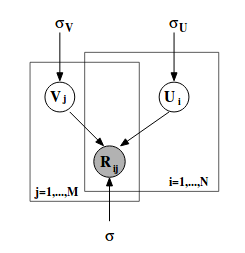
\includegraphics[width=60mm]{pmf-model}
\end{figure}
The conditional distribution over the observed ratings are:
\begin{equation}
	P(R | U, V, \sigma^2) = \overset{N}{\underset{i=1}{\prod}}\overset{M}{\underset{j=1}{\prod}}[N(R_{ij} | U_i^TV_j, \sigma^2)]^{I_{ij}}
\end{equation}
And the conditional distribution over the user and movie feature vectors are:
\begin{equation}
	\begin{split}
		P(U | \sigma^2_{U}) &= \overset{N}{\underset{i=1}{\prod}}N(U_i|0, \sigma^2_{U})\\
		P(V | \sigma^2_{V}) &= \overset{M}{\underset{j=1}{\prod}}N(V_j|0, \sigma^2_{V})\\
	\end{split}
\end{equation}
The log of the posterior over the user and movie feature matrices are given as:
\begin{equation}
\begin{split}
	\ln P(U, V | R, \sigma^2, \sigma^2_{U}, \sigma^2_{V} ) &= \frac{-1}{2\sigma^2}\overset{N}{\underset{i=1}{\sum}}\overset{M}{\underset{j=1}{\sum}}I_{ij}(R_{ij}-U_i^TV_j)^2-\frac{1}{2\sigma^2_{U}}\overset{N}{\underset{i=1}{\sum}}U_i^TU_i-\frac{1}{2\sigma^2_{V}}\overset{M}{\underset{j=1}{\sum}}V_j^TV_j\\
	&-\frac{1}{2}((\overset{N}{\underset{i=1}{\sum}}\overset{M}{\underset{j=1}{\sum}}I_{ij})\ln \sigma^2 + Nk\ln \sigma^2_U+Mk\ln \sigma^2_V) + C
\end{split}
\end{equation}
Maximizing the log posterior with respect to the user and movie feature matrices while keeping the covariance on user and movie features fixed is equivalent to minimizing he sum-of-squared errors objective function with quadratic regularization term as follows:
\begin{equation*}
	E  = \frac{1}{2}\overset{N}{\underset{i=1}{\sum}}\overset{M}{\underset{j=1}{\sum}}I_{ij}(R_{ij}-U_i^TV_j)^2 + \frac{\lambda_U}{2}\overset{N}{\underset{i=1}{\sum}}\rVert U_i \rVert^2 + \frac{\lambda_V}{2}\overset{M}{\underset{j=1}{\sum}}\rVert V_j \rVert^2
\end{equation*}
where $ \lambda_U = \sigma^2/\sigma_U^2 $ and $ \lambda_V = \sigma^2/\sigma_V^2 $ which are effectively kept as constants. One problem that naturally arises with this formulation is that the inner product $ U_i^TV_j $ might be out of the normal rating range (0 to 5 for our dataset). One solution is to replace the product $ U_i^TV_j $ with $ g(U_i^TV_j) $ where $ g $ is the sigmoid function and appropriately scale the original rating with $ t(x) = (x-1)/(S-1) $ where $ S $ is the maximum score. Hence, we modify the above error function as:
\begin{equation}
E  = \frac{1}{2}\overset{N}{\underset{i=1}{\sum}}\overset{M}{\underset{j=1}{\sum}}I_{ij}(t(R_{ij})-g(U_i^TV_j))^2 + \frac{\lambda_U}{2}\overset{N}{\underset{i=1}{\sum}}\rVert U_i \rVert^2 + \frac{\lambda_V}{2}\overset{M}{\underset{j=1}{\sum}}\rVert V_j \rVert^2
\end{equation}
There is no close form solution for $ U $ and $ V $ and thus we use gradient descent to iteratively update $ U_i $ and $ V_j $ until convergence.

One of the main question when using MAP estimation is how should we determine the hyperparameters $ \sigma_U $ and $ \sigma_V $. An 'optimal' choice for these parameters would require looking at the performance on the test set and choose the corresponding parameters values that give the best performance. However, this would mean we need to repeat this algorithm over the search space. One solution is to use the value of the learned variance produced by Variational Bayes method (as we will discuss shortly). Lim and Teh [3] found that this choice of variance parameters works well empirically.

\subsection{Variational Bayes}
One problem associated with the probabilistic matrix factorization method outlined in the previous subsection is over-fitting as MAP is a point estimate and does not account for the variance and uncertainty in the data. Variational Bayes [3], instead of finding just the MAP estimate for $ U $ and $ V $ tries to learn the posterior distribution over $ U $ and $ V $. Variational Bayes (VB) assumes a similar graphical model to PMF where the conditional distribution of the rating is:
\begin{equation*}
P(R | U, V, \sigma^2) = \overset{N}{\underset{i=1}{\prod}}\overset{M}{\underset{j=1}{\prod}}[N(R_{ij} | U_i^TV_j, \sigma^2)]^{I_{ij}}
\end{equation*}
And we also place independent priors on each user and movie feature vectors $ U_i \sim N(0, \sigma_U^2) $ and $ V_j \sim N(0, \sigma_V^2) $. The variational free energy of this model is given as:
\begin{equation}
	L(Q(U, V)) = \E_{Q(U,V)}\log p(R, U, V)-\log Q(U,V)\\
\end{equation}
This is a lower bound on the log likelihood $ \log p(R) $ for all distribution $ Q(U,V) $. Maximizing this lower bound is achieved at $ Q(U,V) = p(U,V,R) $. To make this problem tractable, we use the assumption that the distribution $ Q(U,V) $ factorizes into $ Q(U)Q(V) $. Each distribution also factorizes into the product of the distribution over each user (or movie) feature vector. To be discrete, plugging in the model for $ p(R,U,V) $ yields the full expression for the variational lower bound as follows:
\begin{equation*}
\begin{split}
	L(Q(U)Q(V) &= \underset{Q(U)Q(V)}{E}[\frac{-1}{2}(\overset{N}{\underset{i=1}{\sum}}\overset{k}{\underset{l=1}{\sum}}\log(2\pi\sigma_U^2) + \frac{U_{il}^2}{\sigma_U^2}) - \frac{1}{2}(\overset{N}{\underset{i=1}{\sum}}\overset{k}{\underset{l=1}{\sum}} \log(w\pi\sigma_V^2) + \frac{V_{il}^2}{\sigma_V^2}) \\ &-\frac{1}{2}(\underset{ij}{\sum}\log(2\pi \sigma^2) + \frac{(R_{ij}-U_i^TV_j)^2}{\sigma^2} ) - \log(Q(U)) -\log(Q(V))]\\
	&= \frac{-K}{2}\log(w\pi\sigma^2)-\frac{I}{2}\overset{k}{\underset{l=1}{\sum}}\log(w\pi\sigma_U^2)-\frac{M}{2}\overset{k}{\underset{l=1}{\sum}}\log(w\pi\sigma_V^2)\\
	&-\frac{1}{2}\overset{k}{\underset{l=1}{\sum}}( \frac{\overset{N}{\underset{i=1}{\sum}}E_{Q(U)[U_{il}^2] } }{\sigma_U^2} +\frac{\overset{M}{\underset{j=1}{\sum}} E_{Q(V)}[V_{jl}]^2 }{\sigma_V^2} )\\
	&-\frac{1}{2}\underset{ij}{\sum} \frac{E_{Q(V)Q(V)}[(R_{ij}-U_i^TV_j)^2]}{\sigma^2}
\end{split}
\end{equation*}
%In mean field  where the solution is:
%\begin{equation*}
%	Q^*(U) = \underset{V}{\E} \log p(R,V,\sigma^2,\sigma_U^2,\sigma_V^2)
%\end{equation*}
The solutions for $ Q(U) $ and $ Q(V) $ are obtained by setting the partial derivatives with each to 0 and solve the corresponding equation. The form for $ Q^*(V) $ is similarly defined. Note that this is an iterative algorithm where we update the distribution for $ Q(U) $ and $ Q(V) $ until convergence. The distribution for $ Q^*(U) $ and $ Q^*(V) $, however, are product Gaussian distributions over their feature vectors and have the following closed form:

\begin{equation}
\begin{split}
Q(U) &\propto \overset{N}{\underset{i=1}{\prod}} \exp -\frac{1}{2} (U_i- \bar{U_i})^T \Phi_i^{-1}(U_i-\bar{U_i})\\
	\Phi_i &= \text{inv}(\text{diag}(\frac{1}{\sigma_U^2}) +\underset{j \in I(i)}{\sum} \frac{\Psi_j+V_j\bar{V_J}^T}{\sigma^2} ) \\
	\bar{U_i} &= \Phi_i(\underset{j \in I(i)}{\sum}\frac{R_{ij}\bar{V_j}}{\sigma^2})
\end{split} 
\end{equation}
where $ I(i) $ denotes the set of $ j $ indices where $ I_{ij} = 1$ (or simply the non-zero entries of the i'th row of $ I $). The formulation for $ Q(V) $ is similarly defined as:
\begin{equation}
\begin{split}
Q(V) &\propto \overset{M}{\underset{j=1}{\prod}} \exp -\frac{1}{2} (V_j- \bar{V_j})^T \Psi_j^{-1}(V_j-\bar{V_j})\\
\Psi_i &= \text{inv}(\text{diag}(\frac{1}{\sigma_V^2}) +\underset{i \in I(j)}{\sum} \frac{\Phi_i+U_i\bar{U_i}^T}{\sigma^2} ) \\
\bar{V_i} &= \Psi_i(\underset{i \in I(j)}{\sum}\frac{R_{ij}\bar{U_i}}{\sigma^2})
\end{split} 
\end{equation}
We could see the natural formulation of an iterative method that updates the distributions $ Q(U) $ and $ Q(V) $. In fact, we can also find the update rules for the variance parameters by setting the partial derivative of $ L(Q(U),Q(V) $ with respect to these parameters to 0 and solve. These updates are:
\begin{equation}
\begin{split}
(\sigma_U^2)_l &= \frac{1}{N-1} \overset{N}{\underset{i=1}{\sum}} (\Phi_i)_{ll} + \bar{U_{il}}^2\\
(\sigma_V^2)_l &= \frac{1}{M-1} \overset{M}{\underset{j=1}{\sum}} (\Psi_j)_{ll}+\bar{V_jl}^2\\
\sigma^2 &= \frac{1}{K-1} \underset{ij}{\sum} R_{ij}^2-2R_{ij}\bar{U_i^TV_j}+Tr[(Phi_i+\bar{U_iU_i^T})(\Psi_j+\bar{V_jV_j^T})]\\
\end{split}
\end{equation}

\subsection{Monte Carlo Markov Chain}
While the Variational Bayes method, particularly mean field approximation, outlined above has been used with great success in different problems, one inherent limitation of the method is the factorization of the posterior distribution $ Q(U,V) $ into $ Q(U) $ and $ Q(V) $. Therefore, the distribution computation, though tractable, does not produce the exact solution. On the other hand, sampling methods use approximations that, under the assumption of infinite computation resources, can produce the exact value for the distribution $ Q(U,V) $. One of such methods is Monte Carlo Markov Chain. 

Salakhuditnov and Mnih [4], in their paper, used sampling methods to evaluate the posterior $ P(U,V) $. The authors used the following graphical model.
\begin{figure}[H]
	\centering
	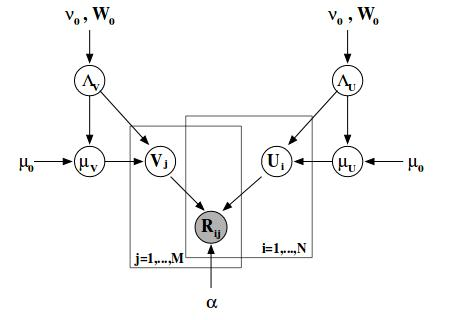
\includegraphics[width=80mm]{mcmc-model}
\end{figure}
where the user and movie feature vectors are assumed to be Gaussian:
\begin{equation*}
\begin{split}
	p(U | \mu_U, \Lambda_U) &= \underset{i=1}{\overset{N}{\prod}} N(U_i | \mu_U, \Lambda_U^{-1})\\
	p(V | \mu_V, \Lambda_V) &= \underset{j=1}{\overset{M}{\prod}} N(V_j | \mu_V, \Lambda_V^{-1})\\
\end{split}
\end{equation*}
In addition, we also place a Gaussian-Wishart distribution on the user and movie hyper-parameters $ \Theta_U ={\mu_U, \Lambda_U} $ and $ \Theta_V ={\mu_V, \Lambda_V} $ as:
\begin{equation*}
\begin{split}
	p(\Theta_U|\Theta_0) &= p(\mu_U|\Lambda_U)p(\Lambda_U) = N(\mu_U|\mu_0, (\beta_0\Lambda_U)^{-1})W(\Lambda_U|W_0,\nu_0)\\
	p(\Theta_V|\Theta_0) &= p(\mu_V|\Lambda_V)p(\Lambda_V) = N(\mu_V|\mu_0, (\beta_0\Lambda_V)^{-1})W(\Lambda_V|W_0,\nu_0)\\
\end{split}
\end{equation*}
where the Wishart distribution is a two parameter distribution given by a scalar $ \nu_0 $ degrees of free dom and a $ k \times k $ scale matrix $ W_0 $:
\begin{equation*}
	W(\Lambda|W_0, \nu_0) = \frac{1}{C}|\Lambda|^{(\nu_0-k-1)/2} \exp(\frac{-1}{2}Tr(W_0^{-1}\Lambda))
\end{equation*}
And C is the normalizing constant. For our purposes, $ \nu_0 $ is set to $ k $ and $ W_0 $ is the identity matrix.

To produce good predictions over unobserved data, we want to approximate the predictive distribution. $ P(R^*_{ij}|R, \Theta) =\int\int p(R^*_{ij}|U_i V_j) p(U, V| R, \Theta) p(\Theta) d\Theta_U d\Theta_V $. However, the exact form for this distribution is analytically intractable. As a result, we use sampling methods to approximate this distribution. MCMC-based methods use Monte Carlo approximations to the predictive distribution as:
\begin{equation*}
	p(R^*_{ij}|R, \Theta_0) \approx \frac{1}{T}\overset{T}{\underset{t=1}{\sum}} p(R^*_{ij}|U_i^t, V_j^t)
\end{equation*}
where $ T $ is the number of samples that we generate using MCMC. In our problem, we will use Gibbs sampling which cycles through the latent variables, sampling each one from the distribution conditional on the current values of all other variables. Because of our choice of the prior distributions, the distributions that we want to sample from all have closed form that are convenient to work with.

In particular, the distribution over the user and movie features are both Gaussians:
\begin{equation}
\begin{split}
	p(U_i | R, V, \Theta_U, \alpha) &= N(U_i |\mu_i^*, (\Lambda^*_i)^{-1})\\
	&\sim \underset{j}{\prod} N(R_{ij}|U_i^TV_j, \alpha^{-1}) p(U_i|\mu_U, \Lambda_U)
\end{split}
\end{equation}
where
\begin{equation*}
\begin{split}
	\Lambda^*_i &= \Lambda_U + \alpha \overset{M}{\underset{j=1}{\sum}}[V_jV_j^T]^{I_{ij}}\\
	\mu_i^* &= [\Lambda_i^*]^{-1} \alpha \overset{M}{\underset{j=1}{\sum}}([V_jR_{ij}]^{I_{ij}} + \Lambda_U \mu_U)
\end{split}
\end{equation*}
The form for the movie feature vectors are very similar and is omitted here for brevity. Furthermore, we can also have a closed form for the hyperparameters over the feature matrices. In fact, these distributions are Gaussian-Wishart given as:
\begin{equation}
	p(\mu_U, \Lambda_U|U, \Theta_0) = N(\mu_U|\mu_0^*, (\beta_0\Lambda_U)^{-1})W(\Lambda_U|W^*_0,\nu^*_0)
\end{equation}
where
\begin{equation*}
\begin{split}
\mu^*_0 &=\frac{\beta_0\mu_0+N\bar{U}}{\beta_0+N}\\ \beta^*_0 &= \beta_0 + N\\
\nu^*_0 &= \nu_0 + N\\
[W_0^*]^{-1} &= W_0^{-1} + N\bar{S} + \frac{\beta_0 N}{\beta_0 + N}(\mu_0-\bar{U})(\mu_0-\bar{U})^T\\
\bar{U} &= \frac{1}{N}\sum U_i\\
\bar{S} &= \frac{1}{N}\sum U_iU_i^T
\end{split}
\end{equation*}
Once again, the form for the distribution over the hyperparameters for $ V_j $  looks similar and thus is omitted for brevity. Hence, with all the distributions derived, the Gibbs sampling algorithm proceeds as follows:\\

\begin{algorithm}[H]
	\caption{Gibbs sampling for Bayesian PMF}
	\begin{algorithmic}
	\STATE 1. Initialize model parameters ${U^1, V^1}$ \\
	\STATE 2. For t = 1, ..., T \\
	\STATE \hspace{2em} Sample hyperparameters according to (12):
	\STATE \hspace{4em} $ \Theta_U^t \sim p(\Theta_U|U^t, \Theta_0) $
	\STATE \hspace{4em} $ \Theta_V^t \sim p(\Theta_V|V^t, \Theta_0) $
	\STATE \hspace{2em} For i = 1 to N, sample user feature vector according to (11):
	\STATE \hspace{4em} $ U_i^{t+1} \sim p(U_i | R, V^t, \Theta_U^t) $
	\STATE \hspace{2em} For j = 1 to M, sample movie feature vector similar to (11):
	\STATE \hspace{4em} $ V_j^{t+1} \sim p(V_j|R,U^{t+1},\Theta_V^t) $\\
	3. Produce prediction for unobserved ratings:
	\STATE \hspace{2em} $ R^*_{ij} = \frac{1}{T}(U^T_i)^TV^T_j $
	\end{algorithmic}
\end{algorithm}

\section{Experiment and data}

The data set used in my experiments is taken from MovieLens-100k data set. The data set has already been divided into training and test set. I ran the different algorithms on the training set and measure MSE performance on the test set. The dataset contains 943 users and 1680 movies. The ranks being experimented on are $ = 5, 10 $ and $ 15 $. I ran all algorithms over 75 iterations and measure the MSE on the test set at each iteration. 

\section{Results}
The following figures show the results of the experiments. In practice, the choice of rank to decompose with is problem specific. It is often the case that we need to perform a grid search over the possible values of k to determine the value giving the lowest MSE. 

\begin{figure}[H]
	\centering
	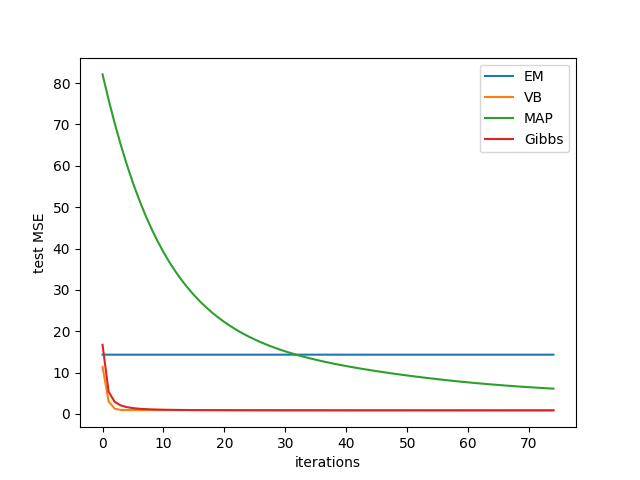
\includegraphics[width=150mm]{rank_5.png}
	\caption{Rank 5 factorization}
\end{figure}

\begin{figure}[H]
	\centering
	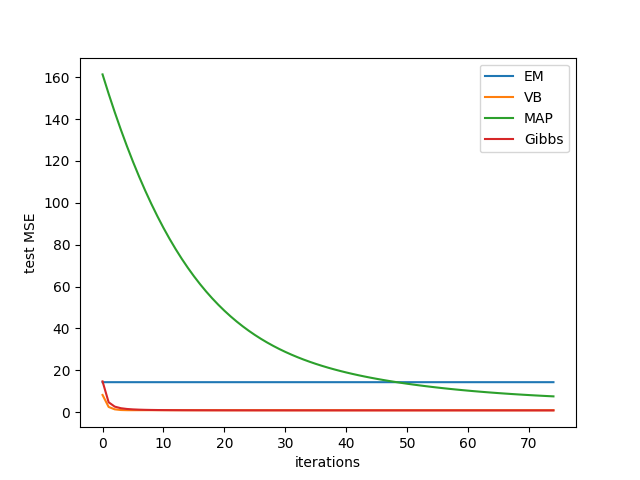
\includegraphics[width=150mm]{rank_10.png}
	\caption{Rank 10 factorization}
\end{figure}

\begin{figure}[H]
	\centering
	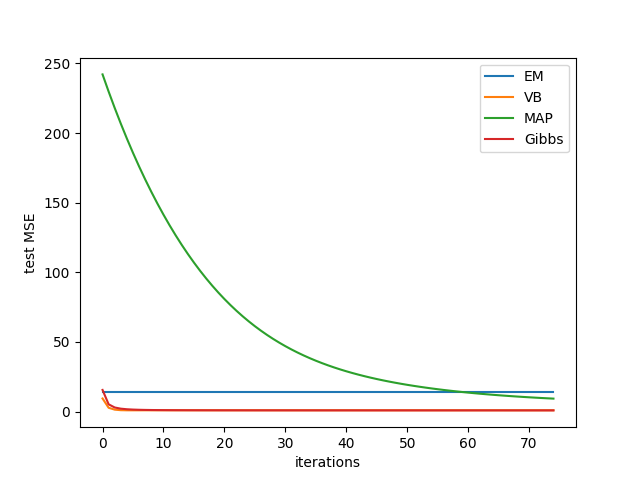
\includegraphics[width=150mm]{rank_15.png}
	\caption{Rank 15 factorization}
\end{figure}

\section{Discussion}
We can see from the above plots that Variational Bayes and Gibbs Samplings handily beat both EM and MAP algorithms in terms of test set MSE. Both algorithms converge within much fewer iterations than the other two algorithms.

It's worth noting that SVD seems to stay pretty much 'flat' throughout all the iterations. In reality, SVD doesn't produce a constant estimates but rather makes very little improvement. As a result, when plotted against other algorithms, it really highlights that SVD doesn't make much improvements. Because the EM algorithm used is a naive version and unweighted, the true potential of EM-SVD was not realized. This could be left for future work.

MAP algorithm does make significant improvements over many more iterations. However, the convergence is a lot slower than VB and Gibbs samplings. Furthermore, MAP requires a good choice of hyperparameters to fully realize is potential. In this experiment, the starting point for MAP was chosen by the variances produced by VB. However, more time was needed to verify whether this choice of variances parameters was optimal. However, a quick comparisons with other choices for variancse show that VB estimates for variance were relatively good.

Gibbs and VB have very similar performance. Although not clear on the graph, numerical results show that Gibbs tend to edge out slightly better than VB. From a theoretical stand point, this makes sense because Gibbs sampling produce approximations that asymptotically converge to the correct distributions while VB produces an inexact, though tractable solutions. Furthermore, comparing two algorithms just in terms of MSE is inadequate as two algorithms have different strengths. While Gibbs give theoretically better results, sampling methods are often avoided because of their computational cost so sampling methods will not work well on large scale problem. On the other hand, VB produces inexact approximations that might not be as good as Gibbs in small scale problems but this inexact approximation allows it to scale to larger size problems.
 
\section{Conclusion}

The results of the experiments allow us to have a good idea of the relative performances among the different algorithms in the matrix factorization problem (particularly the movie rating prediction problem). It seems that Gibbs samplings and VB should be the method of choices for matrix completition problems over MAP and SVD-EM. One of the main limitations of the experimentation is the scale of the problem. 943 users and 1680 movies is a very modest size for matrix completition problem. In comparison, the netflix data set contains over 400,000 users and 17,000 movies and over a million ratings. However, due to the limited time and inefficiency of the code, a smaller data set has to be used to produce meaningful results presented in this report. One of the possible future works would certainly be testing and comparing these different algorithms on larger data sets as well as large synthetic data sets.

\begin{thebibliography}{}
	\bibitem{em-svd} 
	Nathan Srebro, Tommy Jaakkola 
	\textit{Weighted Low Rank Approximations}. 
	ICML, 2003.
	
	\bibitem{pmf} 
	Ruslan Salakhutdinov, Andriy Mnih 
	\textit{Probabilistic Matrix Factorization}
	
	\bibitem{pmf} 
	Yew Jin Lim, Yee Whye Teh 
	\textit{Variational Bayesian Approach to Movie Rating Prediction}

	\bibitem{pmf} 
	Ruslan Salakhutdinov, Andriy Mnih 
	\textit{Bayesian Probabilistic Matrix Factorization using Markov Chain Monte Carlo}
\end{thebibliography}


\end{document}



